%!TEX root = ../main.tex

\chapter{Measurements\label{chap:measurements}}

\section{Equipment}

The event based camera used in this work is the model EVK4\footnote{Prophesee EVK4 website: \url{https://www.prophesee.ai/event-camera-evk4/}.}, manufactured by Prophesee. The camera has a resolution of 
$1280 \times 720$ pixels, with maximum frame rate equivalent of 10k fps and a dynamic range of 120 dB.
A fish eye lens with an inbuilt UV filter was used during the measurements to target the specific wavelength of the LEDs
that are used on the UAVs. The camera is shown on \reffig{fig:evk4}. 

% \begin{figure}[htbp]
%   \centering
%   \subfloat[EVK4 event-based camera.] {
%     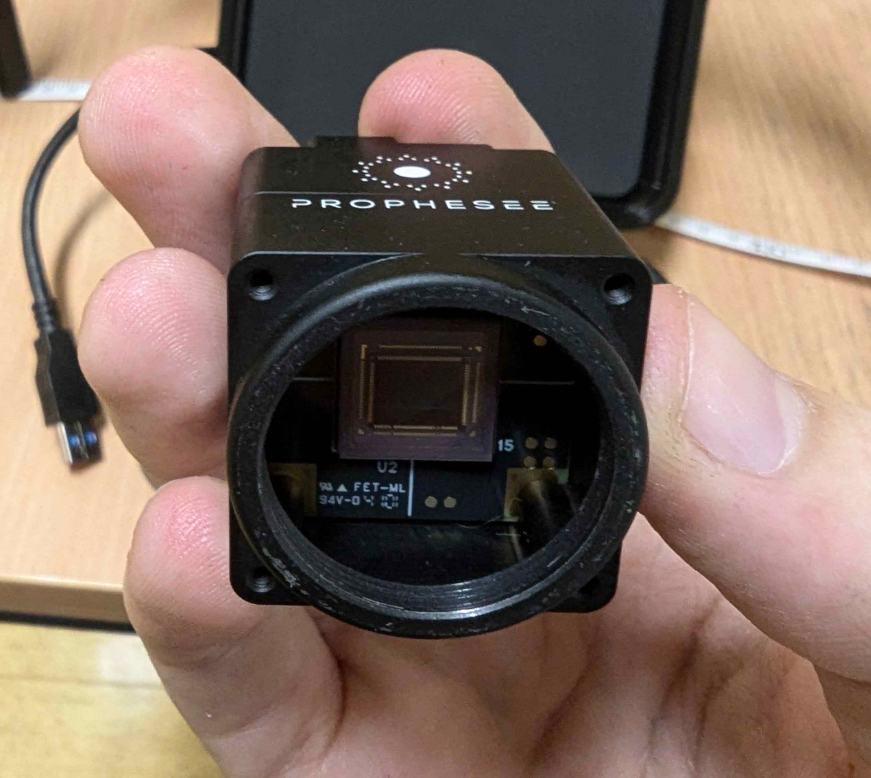
\includegraphics[width=0.3\textwidth]{./fig/photos/evk4.png}
%     \label{fig:evk4_1}
%   }
%   \subfloat[EVK4 event-based camera with a fish eye lens.] {
%     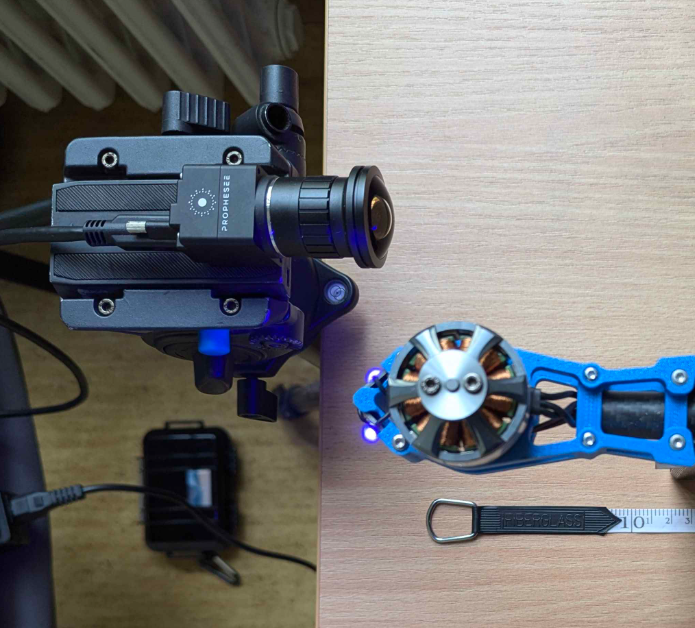
\includegraphics[width=0.3\textwidth]{./fig/photos/lens.png}
%     \label{fig:evk4_2}
%   }
%   \caption{
% The event based camera EVK4 from Prophesee, on \reffig{fig:evk4_1}, with a fish eye lens on \reffig{fig:evk4_2}.
% }
%   \label{fig:evk4}
% \end{figure}

\begin{figure}[htbp]
	\centering
	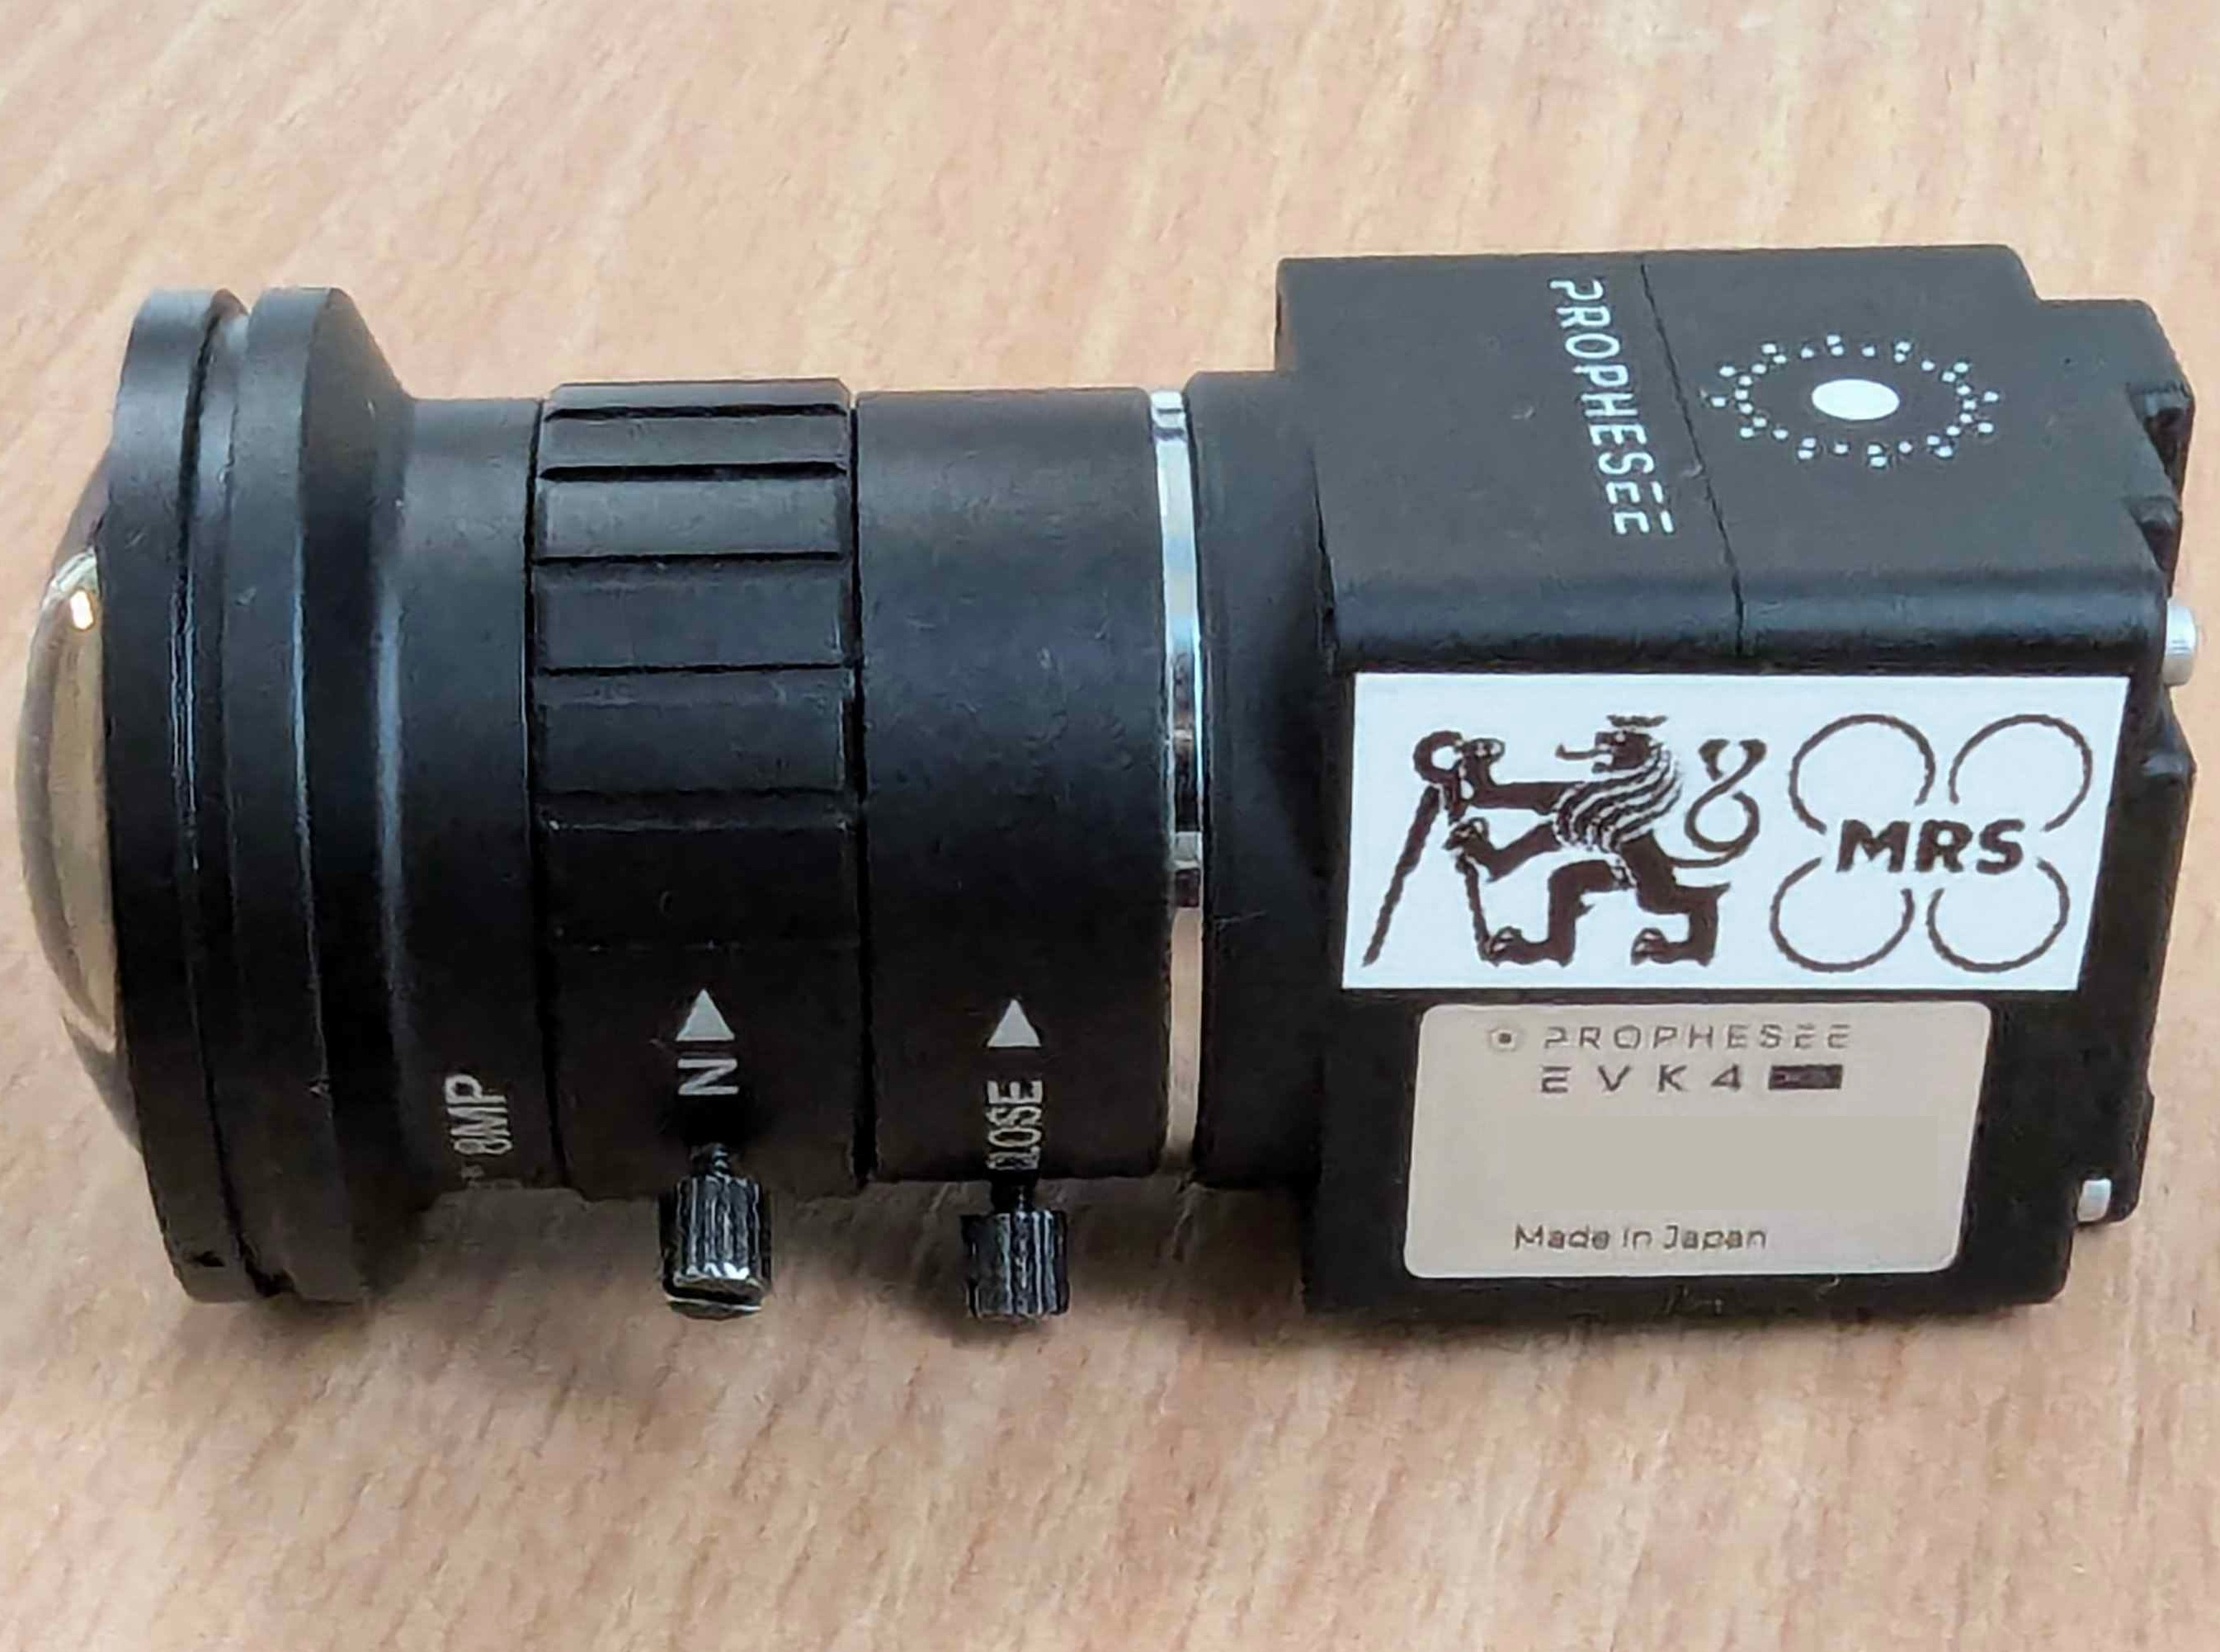
\includegraphics[width=0.50\textwidth]{./fig/photos/camera_with_lens.jpg}
	\caption{The event based camera EVK4 from Prophesee with a 2.5mm F1.6 fish eye lens.}
	\label{fig:evk4}
\end{figure}

The data from the camera has been obtained using the Metavision Studio software, which records the data in the .raw format.
Data is then later processed using various functions of the Metavision SDK\footnote{Metavision SDK Docs: \url{https://docs.prophesee.ai/stable/index.html}},
which has either C++ or Python API. In this work, the Python API has been used.

\section{Data collection}

The data has been collected on several occasions by measuring a stationary UAV which is a part of the MRS UVDAR system, that
uses UV \ac{LED} sources for localization and communication between individual UAVs. 
Each UAV is equipped with 8 UV LEDs, with 2 LEDs on each arm of the UAV. Each of the LEDs can be individually controlled
and can be set to various sequences of blinking (not only on/off).

\subsection{Initial measurements}

The initial measurements were done by securing the event camera on a tripod and placing the UAV at distances ranging from
$0.5$ to $2.5$ meters. The LEDs were set to blink at a frequency in range of $1$ Hz to $30$ kHz. No \ac{ROI} was set
and the whole image has been recorded during the testing.

This first experiment proved to be rather inefficient, as the LEDs need to be isolated from each other's influence, which
was not done properly at this time. This problem is solvable in the post processing, by filtering out the events
by using a ROI filter, but this proved rather inefficient (it is possible to filter the events by finding bounding boxes
that encapsulate light sources, but on a more complex scene this approach becomes relatively hard).
The other issue turned out to be the reflections of surrounding objects (as seen on \reffig{fig:meas1}), which caused
another source of unwanted events in the recording.

\begin{figure}[htbp]
  \centering
  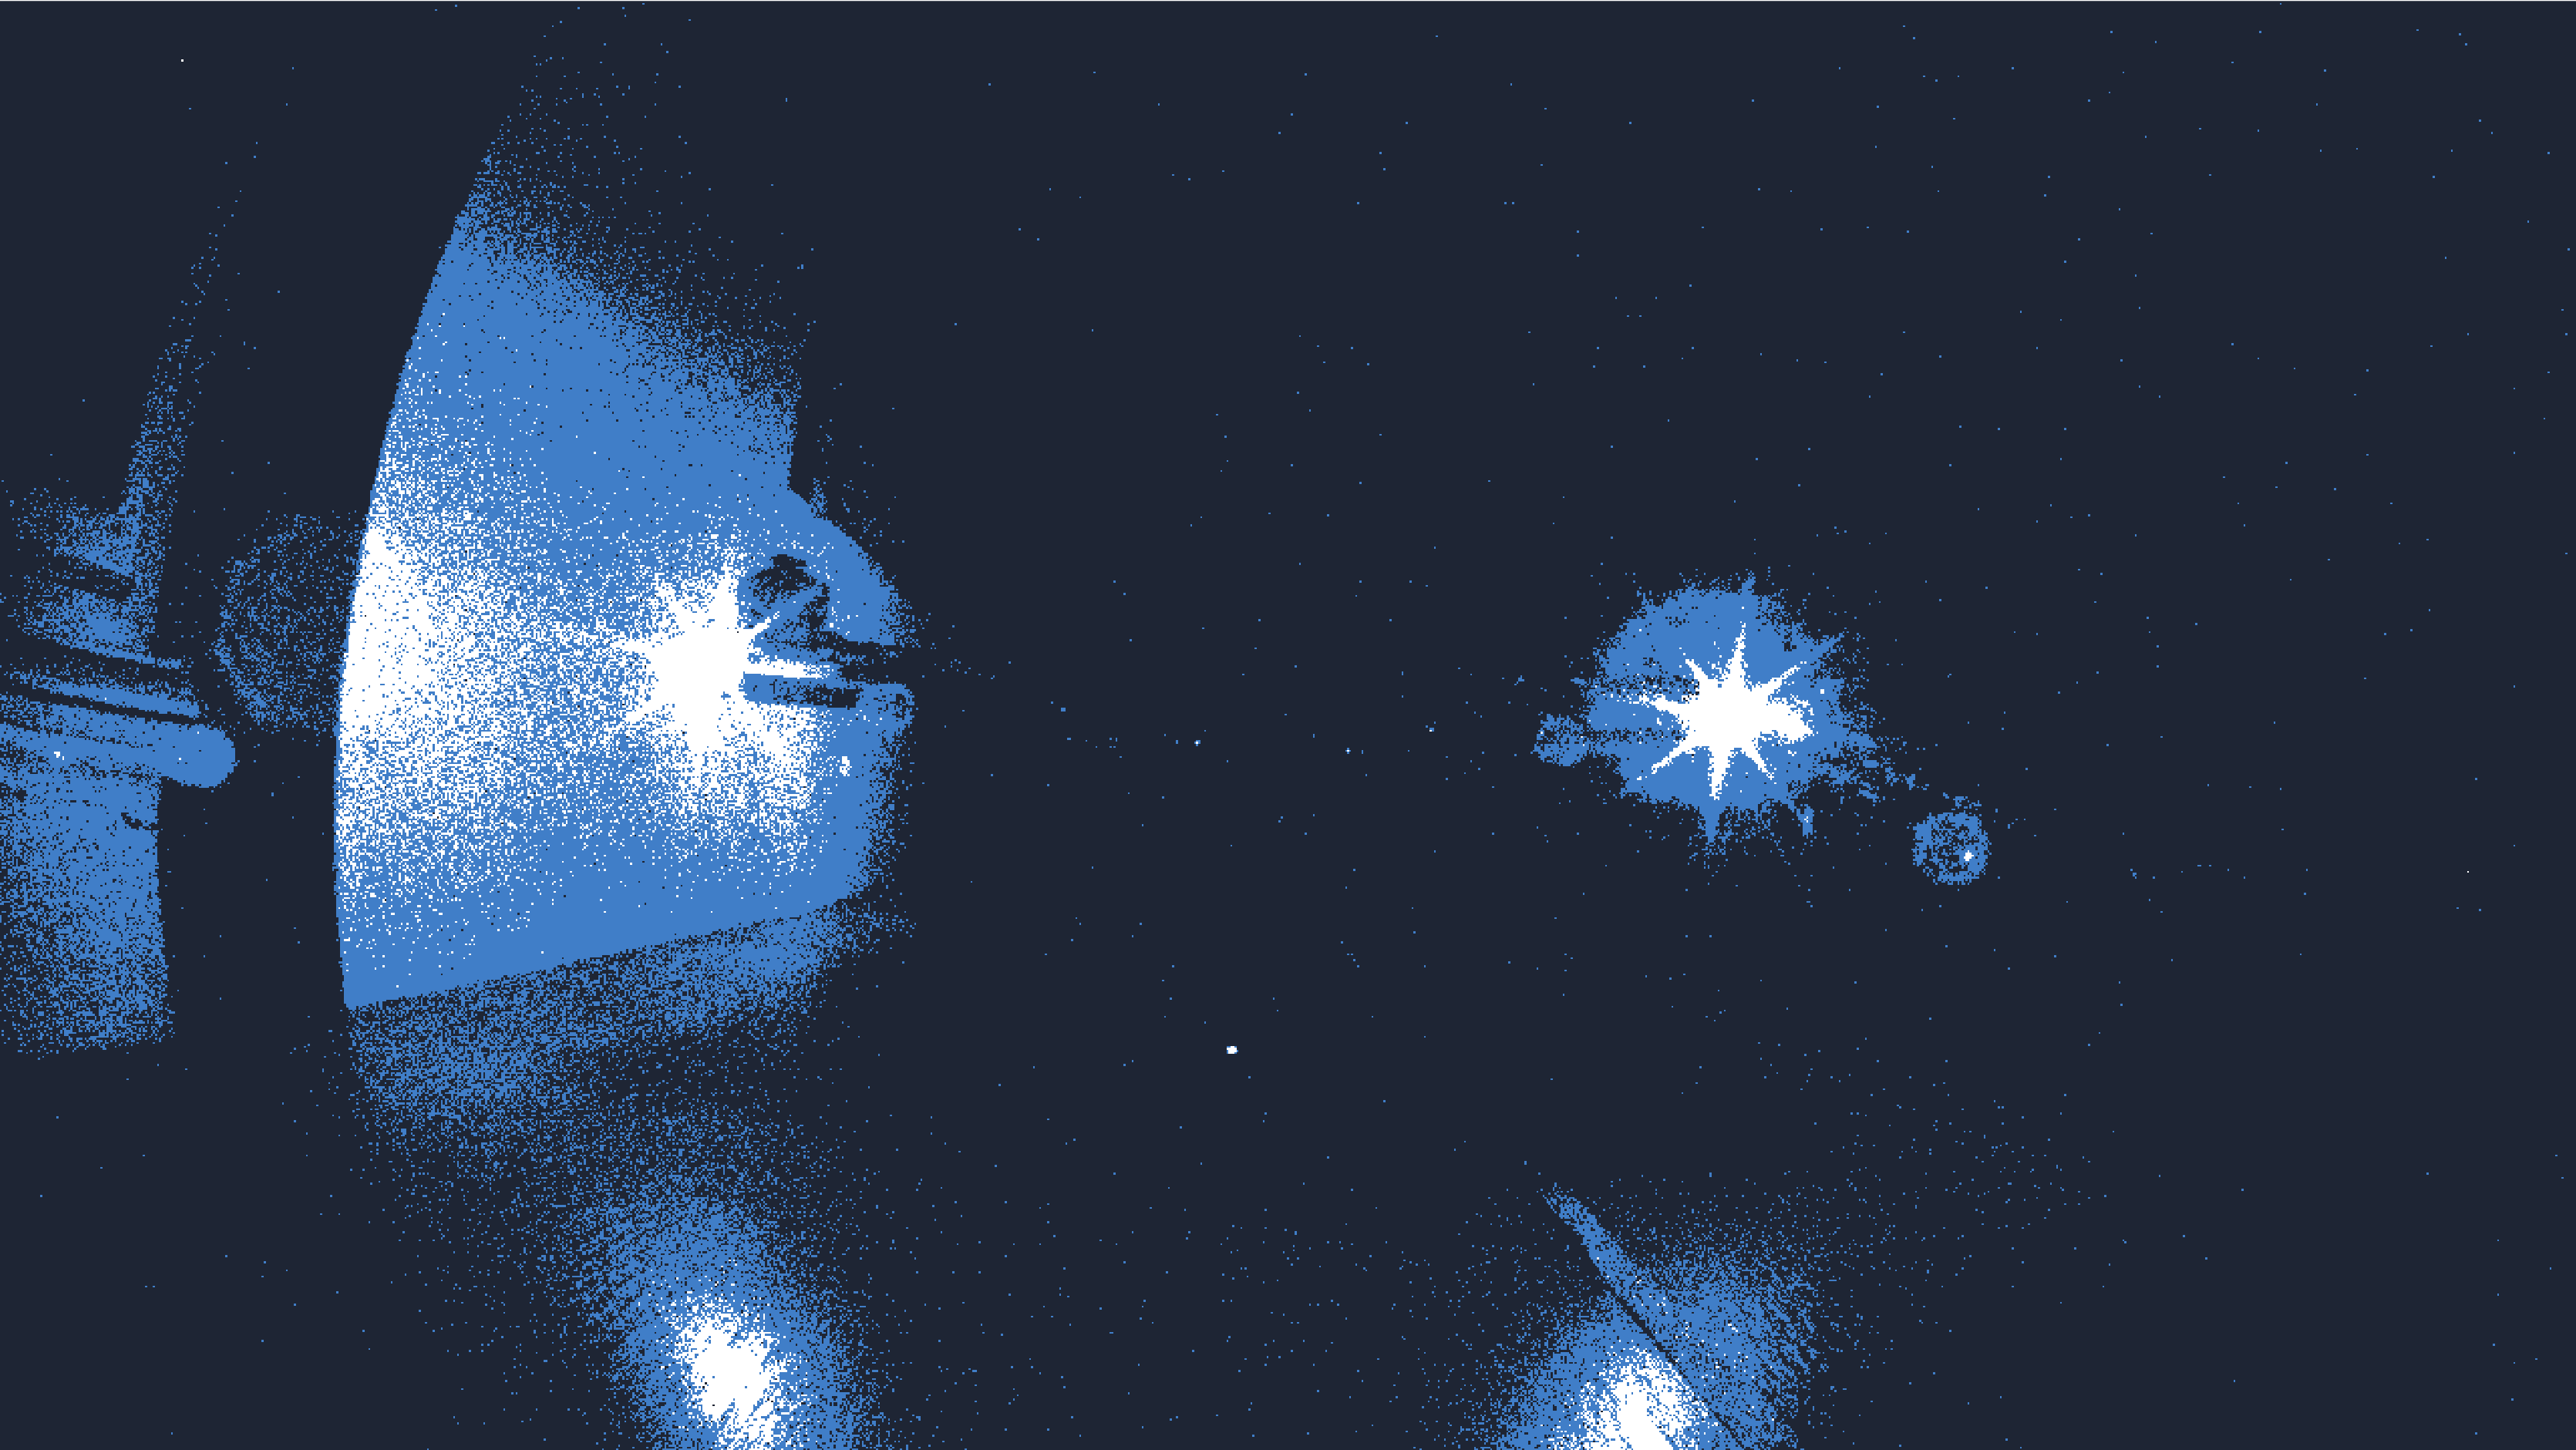
\includegraphics[width=0.5\textwidth]{./fig/photos/meas1.png}
  \caption{Visible reflections can be seen on the wall on the left side of the image.}
  \label{fig:meas1}
\end{figure}

\subsection{Distance - frequency influence}

In the following measurements, we consider one source of light as the whole arm of the UAV (with 2 UV LEDs). Measurements were
done on areas isolated by ROI filter directly in Metavision Studio - events were collected only on a select area, with the
rest of the events being discarded.
This time, the position of the UAV was fixed relative to the camera on a blank background. The camera was placed on a tripod
and moved by increments of $0.2$ meters, starting from $1$ meter and ending at $3$ meters, with additional measurements done
at $4$ and $5$ meters.

Frequency range of the LED modulation was set in a range from $10$ Hz to $30$ kHz.

\subsection{Rotation angle influence}

In addition to a distance and frequency influence, the rotation angle influence also needs to be considered, to
verify the emitting characteristics of the light sources - if they can or cannot be considered lambertian.
The UAV was rotated by increments of $45$ degrees relative to the event camera, at distances of $0.5$, $1$ and $2$ meters,
with frequencies ranging from $10$ Hz to $10$ kHz. 

\subsection{RSSR Data collection}

Another dataset will be collected for the application of \ac{RSSR} \cite{bai2021vlp},
which will serve as the focus of the subsequent bachelor thesis that builds upon this semester project.